\documentclass[12pt]{article}
\usepackage{setspace}
\doublespacing
\usepackage[margin=0.5in]{geometry}
\usepackage{rotating} % rotate figures to landscape view
%\usepackage[top=15pt, bottom=10pt, left=20pt, right=20pt]{geometry}
\usepackage[toc,page]{appendix}
\usepackage{cancel,comment,alltt}
\usepackage{mathtools,amsmath,amsthm,bm,amsfonts}

\usepackage{url,hyperref,breakurl}

\usepackage{float,subfig,color,array,multirow,tikz}

\usepackage{multirow}
%\linenumbers


\begin{document}


\subsection{Group}
A group is a set, $\mathbb{G}$, with an operation $*$ that combines two elements $a$ and $b$ to form $a*b$ satisfying:
\begin{itemize}
   \item closure $a*b \in \mathbb{G}$. 
   \item identity $e \in \mathbb{G}$ such that $e*a = a*e = a$. 
   \item existence of an inverse $b \in \mathbb{G}$ such that $a*b = b*a = e$. 
   \item associativity $(a*b)*c = a*(b*c)$. 
\end{itemize}

{\bf Example}: Exibit the group structure of a parabola $y= x^2$ with parametrization $\alpha(x)= [x,x^2]$. \\
proof:
The identity is the origin $(0,0)$.
$a*b$ is the intersection of the line through $(0,0)$ parallel to $\overline{ab}$ on the parabola in $A^2$.
We want to find the point $a*b$ which is the intersection of the line $y=cx$ (with slope $c=(b_2-a_2)/(b_1-a_1)$) for $\overline{ab}$ and $y=x^2$.
Hence, we obtain the intersection from equating $x^2=cx$, which gives $x=c$ and $y=c^2$.
This defines the point $a*b = [(b_2-a_2/(b_1-a_1),(b_2-a_2)^2/(b_1-a_1)^2]$.

\subsection{Translation on a line $A^1$}
A translation $\tau^1$ ($\tau^{-1}$) translates the points of $A^1$ by $1$ to the right (left).
The ``orbit" generated by a point x: x under $\tau^1$ and $\tau^{-1}$ and all iterates on $A^1$.
The circle $S^1$ is the space of all orbits (i.e., the orbit of $x$ and the orbit of $x+1$ is the same orbit)

\subsection{Rational Parametrization (for a unit circle)}

\begin{equation}
   e(m) = ( \frac{1-m^2}{1+m^2}, \frac{2m}{1+m^2} ),
\end{equation}

m is the slope of a line $y=m(x+1)$ that passes through $(-1,0)$ parameterizing the circle.
$m=\infty, e(m) = (-1,0)$. 
$m=0, e(m)=(1,0)$.

\subsection{Transcendental Parametrization}

\begin{equation}
   \psi(\theta) = (\cos(\theta), \sin(\theta))
\end{equation}

\subsection{Projective Space} 
{\bf Def}: Sets of all lines through the origin of a vector space $V$. \\

$P^1(A^2)$ (projective lines) = space of all 1D subspaces of $A^2$

\begin{itemize} 
   \item[1.] A circle $S^1$ is topologically $P^1(R^2)$ $\longrightarrow$ $P^1 \simeq S^1$.
   \item[2.] A sphere $S^2$ is topologically $P^1(C^2)$   $\longrightarrow$ $P^1 \simeq S^2$.
\end{itemize}
Proof for 2. 
Suppose we have a lines through the origin of $C^2$, $t(w,k)$, where (w,k) is any vector in $C^2$ and $t \in R$.
When $k \neq 0$, the line divided by k gives $t(w/k,1)$, where $w/k$ is any number in $C$. 
The line $t(w/k,1)$ represents the entire set of lines through the origin except the line $t(w,0)$, when $k=0$, which is defined as the infinity on the complex plane.
As we knew from stereographic projection, the complex plane ($C$) is homeomorphic to the sphere.
Hence, the lines $t(w/k,1)$ with $t(w,0)$ forms the projective line of the sphere $\longrightarrow$ $P^1(C^2) \simeq S^2$.

\subsection{Homeomorphism}

{\bf Def}: Two topological spaces are homeomorphism if there exists a continuous bijective function with a continuous inverse function. \\
$f$ is bijective, continuous and $f^-1$ is continuous.


\subsection{Stereographic Projection P}

Any point on a sphere can be represented with a point $[x,y,0]$ on an equatorial plane. 
Starting with the south pole point $[0,0,-1]$, we derive the projection for the sphere,

\begin{equation}
   P(x,y) = (2x/(1+x^2+y^2), 2y/(1+x^2+y^2), (1-x^2-y^2)/(1+x^2+y^2)).
\end{equation}

The south pole $[0,0,-1]$ on the sphere is the infinity point $(\infty,\infty)$ on the equatorial plane. 
This completes the entire plane $\simeq$ sphere. \\

{\bf Remarks}: 1) A line or circle on the equatorial plane is mapped to a circle on the sphere.
2) A conformal is preserved through $P$ (i.e., the angle of two lines on the plane mapped to the sphere preserves this angle)

\subsection{Conformal}
Any two lines meeting at an angle on the equatorial plane preserves the angle when meeting at the projected circles on the sphere.

\subsection{Inversive Geometry}
In Euclidean geometry, a circle $c$ has a inversion map sending points inside $c$ to outside.
$I_c: x \longrightarrow x'$, 
\begin{equation}
   d(o,x)d(o,x')=r^2,
\end{equation}
where $o$ is the origin, and $r$ is the radius.
$c$ is fixed under $I_c$, $I_c$ just maps a point to another point leaving $c$ intact.
The origin $o$ will be sent infinitely far away, so $I_c$ maps $o$ to $\infty$.

{\bf Remarks }: 
\begin{enumerate} 
   \item A line sectioning through $c$ mapped by $I_c$, is a circle through the origin.
   \item A circle in $c$, is mapped by $I_c$ to a bigger circle outside $c$. 
   \item Two circles inside $c$ forming an angle, where the angle is preserved when mapped to the outside circles (i.e., conformal).
\end{enumerate}

\section{Algtop5, 2D objects: Torus and Genus}

\subsection{Translation group}
$\left< \tau \right>$: $\tau^n$ is the translation by an integer $n$, which is a group of transformation of $A$.
$\tau^0$ is the identity, $(\tau^n)^{-1}=\tau^{-n}$.
$O_x$ is the orbit of x, which consist of $\left< \tau \right>$.

A Cylinder is topologically the space of all orbits in $A^2$.

\subsection{Torus}
Doughnut shaped surface $T= S^1 \times S^1$. \\

The number of holes of a torus is defined as ``Genus", g: maximum number of disjoint loops on the surface which do not disconnect the surface. \\

Jordan curve THM: prove that any loop on $S^2$ disconnects $S^2$. \\

The genus of a sphere $g(S^2)= 0$ (i.e., any number of loops will disconnet the sphere into a disk and a sphere with a hole). \\
The genus of a torus $g(T)= 1$ (i.e., one loop cutting the torus into a cylinder does not disconnect the torus). \\
The genus of a 2-hole torus $g(\text{2-hole } T)= 2$ (i.e., also cutting the torus into a cylinder).
  \begin{figure}[H]
     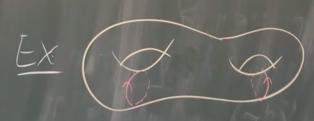
\includegraphics[width=0.5\textwidth]{twoholeT}
  \end{figure}

\subsubsection{Torus as a configuration space}
configuration space $T_1, T_2, r_1, r_2$.
  \begin{figure}[H]
    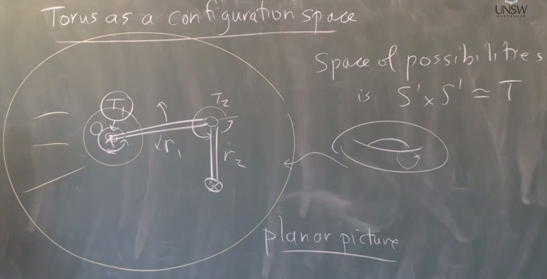
\includegraphics[width=0.5\textwidth]{torus_config_space}
  \end{figure}
    

\subsubsection{Torus as an orbit space}
  Suppose $\tau_1$ ($\tau_2$) is a one translation to the right (up).
  $G= \left< \tau_1, \tau_2 \right>$: group generated by all $\tau_1^n$ and $\tau_2^m$, where $n, m \in Z$, and $G= Z \times Z$.
  Every orbit meets the unit square in 1, 2, or 4 points. 
  Glue the edges together and get a torus.
  \begin{figure}[H]
     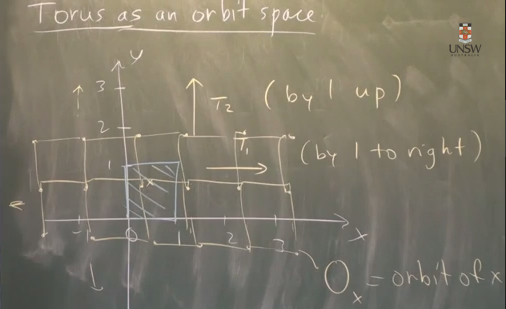
\includegraphics[width=0.5\textwidth]{torus_orbit_space1}
     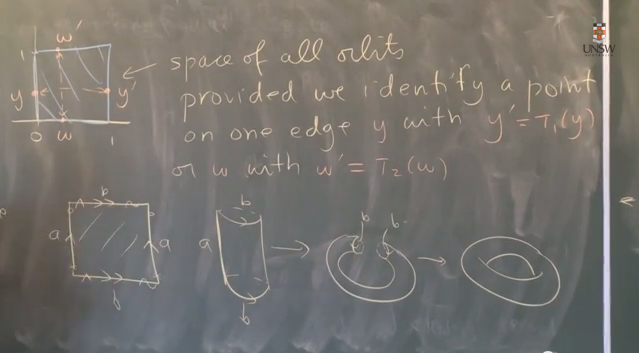
\includegraphics[width=0.5\textwidth]{torus_orbit_space2}
  \end{figure}

\subsection{Tessellation of a plane}
Tessellation: A tiling of regular polygons (2-D), polyheda (3-D), polyhedron/polytope (n-D). \\

{\bf Prob} Show that by gluing a hexagon we get a torus.


\section{Non-orientable surfaces: Mobius band}
{\bf Def}: A surface $M$ is orientable if we can consistently assign a positive rotation as we move among the surface and back to the same starting point. \\

{\bf Example}: A torus is orientable. A positive/counterclockwise rotating loop is always positive when moved among the surface. \\

{\bf Counter Example}: A Mobius band is non-orientable. 
If you move a $x-y$ cross around the band, the $x$ will be pointing in the other direction when it returns to the start.
A man walking with a left-hand up will change to right-hand when completing a cycle. \\

{\bf Application for Mobius band}: A belt around two wheels is twisted to use both sides of the belt => Mobius band! \\

\subsection{Crosscap (self-intersection)} one of the two building blocks for 2D surfaces, the other one is a ``handle".

\sebsection{Classification THM for Surfaces}
Any 2D compact surface is 1) a sphere 2) a finite # of handles (i.e., n-hole torus) 3) a sphere with finite # of crosscaps (i.e., projective plane, Klein bottle, ...).
1 and 2 are orientable, 3 is unorientable.

{\bf Proof:} 


\end{document}
